\documentclass[a4paper, 12pt]{article}

\usepackage[utf8]{inputenc}
\usepackage[T1, T2A]{fontenc}
\usepackage[english, russian]{babel}
\usepackage[top=2cm, bottom=2cm, left=2cm, right=2cm]{geometry}
\usepackage[T2A]{fontenc}
\usepackage[utf8]{inputenc}
\usepackage[english, russian]{babel}
\usepackage[top=2cm, bottom=2cm, right=2cm, left=2cm]{geometry}
\usepackage{amsmath}
\usepackage{graphicx}
\usepackage{subcaption}
\usepackage{float}
\usepackage{tabularx}
\usepackage{pgfplots}
\usepackage{amsmath,booktabs}
\usepackage{array}
\graphicspath{ {images/} }
\usepackage{tabu}
\newcommand\tline[2]{$\underset{\text{#1}}{\text{\underline{\hspace{#2}}}}$}
\usepackage{pgfplots}
\usepgfplotslibrary{polar}
\pgfplotsset{compat=1.13}
\pgfplotsset{grid = major, grid style = {dashed}}

\usepackage{subcaption}
\usepackage{amsmath}

\usepackage{tabu}

\usepackage{float}

% PGFPlots Table ========================================================
\usepackage{pgfplotstable}
\renewcommand{\arraystretch}{1.3}
% recommended:
\usepackage{booktabs}
\usepackage{colortbl}
% pgfplotstable settings
\pgfplotstableset{
    every head row/.style = {before row = \hline},
    after row = {[1mm] \hline},
    column type = {|c},
    every last column/.style={
        column type/.add={}{|},
    },   
}
\usepackage{threeparttable}
\renewcommand{\TPTminimum}{0.6\linewidth}

% Paragraph indent
\usepackage{indentfirst}
\setlength{\parindent}{15mm}

%Change label separator
\usepackage{caption}
\captionsetup[table]{labelformat=simple, labelsep = endash, justification = raggedright, singlelinecheck = off, width = 0.75\textwidth}
\captionsetup[figure]{labelformat=simple, labelsep = endash, name = Рисунок}



\begin{document}
	\parindent=1.27cm
	
\begin{titlepage}
	\centering
	{\fontsize{12pt}{5cm}\selectfont \bfseries Министерство образования и науки Российской Федерации} \\ \vspace{0.5cm}
	{\fontsize{7pt}{5cm}\selectfont ФЕДЕРАЛЬНОЕ ГОСУДАРСТВЕННОЕ АВТОНОМНОЕ ОБРАЗОВАТЕЛЬНОЕ УЧРЕЖДЕНИЕ ВЫСШЕГО ПРОФЕССИОНАЛЬНОГО ОБРАЗОВАНИЯ} \\ 
	\vspace{1cm}
	{\fontsize{12pt}{5cm}\selectfont \bfseries САНКТ-ПЕТЕРБУРГСКИЙ УНИВЕРСИТЕТ ИНФОРМАЦИОННЫХ ТЕХНОЛОГИЙ, МЕХАНИКИ И ОПТИКИ} \\ \vspace{1.5cm}
	
	{\fontsize{14pt}{5cm}\selectfont Кафедра \hspace{1cm} \underline{Систем Управления и Информатики}  \hspace{1cm} Группа \underline{Р3340}} \\ 
	\vspace{2cm}
	
	{\fontsize{20pt}{5cm}\selectfont \bfseries Лабораторная работа №12} \\
	{\fontsize{12pt}{5cm}\selectfont \bfseries “АНАЛИЗ ЛИНЕЙНЫХ НЕПРЕРЫВНЫХ СИСТЕМ С ИСПОЛЬЗО-
		ВАНИЕМ ПРИКЛАДНОГО ПАКЕТА MATLAB CONTROL SYSTEM
		TOOLBOX
		”} \\
	{\fontsize{14pt}{5cm}\selectfont Вариант - 11} \\
	\vspace{1.5cm}
	
	\flushleft
	
	{Выполнил \hspace{2cm} \tline{(фамилия, и.о.)}{9cm} (подпись)} \\
	\vspace{2cm}
	
	{Проверил \hspace{2cm} \tline{(фамилия, и.о.)}{9cm} (подпись)} \\
	\vspace{5cm}
	
	"\underline{\hspace{0.7cm}}"\hspace{0.2cm}\underline{\hspace{2cm}}\hspace{0.2cm}20\underline{\hspace{0.7cm}}г. \hspace{2cm} Санкт-Петербург, \hspace{2cm} 20\underline{\hspace{0.7cm}}г. \\ \vspace{1cm}
	
	Работа выполнена с оценкой \hspace{1cm} \underline{\hspace{8cm}} \\ 
	\vspace{1cm}
	Дата защиты "\underline{\hspace{0.7cm}}"\hspace{0.2cm}\underline{\hspace{2cm}}\hspace{0.2cm}20\underline{\hspace{0.7cm}}г.
	
\end{titlepage}	

\begin{center}
\section{Задача}
\end{center} \par
Целью работы является исследование динамических и частотных характеристик, анализ структурных свойств и устойчивости линейных непрерывных систем с помощью прикладного пакета matlab. \par
В качестве объекта исследования выбраны линейные непрерывные динамические стационарные системы. Исходная модель разомкнутой системы представляется в форме вход-выход и описывается передаточной функцией вида: 
\begin{equation} 
    W(s) = \frac{b_1s + b_0}{s(a_2s^2 + a_1s + a_0)}
\end{equation} \par
Значения коэффициентов $a_0, a_1, a_2, b_0, b_1$ представлены в таблице 1. \par
\begin{table} [h!]
    \centering
    \begin{threeparttable}
        \caption{Коэффициенты передаточной функции}
        \begin{tabular}{|c|c|c|c|c|}
            \hline
            $a_0$ & $a_1$ & $a_2$ & $b_0$ & $b_1$ \\ \hline
            5 & 4 & 3 & 2 & 1 \\ \hline
        \end{tabular}
    \end{threeparttable}
\end{table}
Далее необходимо перейти от исходной разомкнутой системы к замкнутой системе с жесткой отрицательной обратной связью и провести ее анализ в соответствии с порядком выполнения работы.

\newpage
\begin{center}
\section{Анализ разомкнутой системы}
\end{center}

Передаточная функция разомкнутой системы представлена ниже:
\begin{equation}
    W(s) = \frac{s + 2}{3s^3 + 4s^2 + 5s}
\end{equation}

\noindent
\begin{minipage}[t]{0.5\textwidth}
    \begin{figure} [H]
        \centering
        \begin{tikzpicture}
            \begin{axis} [
                width = 0.9\textwidth,
                xlabel = {Re},
                ylabel = {Im},
                grid = major,
                grid style = {dashed},
                legend pos = north west,
            ]
                \addplot[only marks, mark = x, mark size = 5pt] coordinates {(-0.67, 1.105) (-0.67, -1.105) (0, 0)}; 
                \addplot[only marks, mark = o, mark size = 5pt] coordinates {(-2, 0)};
                \legend{полюса, нули};
            \end{axis}
        \end{tikzpicture}
        \caption{Нули и полюса}
    \end{figure}
\end{minipage}
\begin{minipage}[t]{0.5\textwidth}
    \vspace{0.5cm}
    Из исходной системы можем найти нули и полюса.
    \begin{align*}
        p_1 & = -2 \\
        z_1 & = 0 & z_{2, 3} = -\frac{2}{3} \pm i\frac{\sqrt{11}}{3}
    \end{align*}
    где p - полюса, z - нули. Графическое изображение найденых решений представлено на рисунке 1.
\end{minipage}
\vspace{0.5cm} \par

Далее построим логарифмические амплитудночастотные и фазочастотные характеристики. Они представлены на рисунке 2.

\begin{figure}[h!]
	\begin{subfigure}{\textwidth}
	\begin{tikzpicture}
\begin{semilogxaxis} [
width = 0.9\textwidth,
height = 6cm,
ylabel = {$20L(\omega)$, дБ},
xlabel = {$\omega$, 1/c}, grid = major,
grid style = {dashed},
xmin = 10e-2, xmax = 10e+1,
ymin=-100,
extra y ticks = {-20},
extra x ticks = {0.43},
extra x tick labels = {0.43},
xtick = {10e-2, 10e+0, 10e+1, 10e+2},
ytick = {0, 50, -50, -80},
]

\addplot[red, mark=0, thick, smooth, solid] table[x=w, y=lgA] {bode.txt};
\draw[dashed] (0.1, 0) -- (0.43, 0);
\draw[dashed] (0.43, 0) -- (0.43, -180);
\draw[dashed] (2.23, -180) -- (2.23, -20);
\draw (0.43, 0) -- (0.43, 0);
\end{semilogxaxis}
\end{tikzpicture}
\end{subfigure}

\begin{subfigure}{\textwidth}
	\begin{tikzpicture}
	\begin{semilogxaxis} [
	width = 0.9\textwidth,
	height = 6cm,
	ylabel = {$\varphi$, град.},
	xlabel = {$\omega$, 1/c}, grid = major,
	grid style = {dashed},
	xmin = 10e-2, xmax = 10e+1,
	ymin = -210,
	ytick = {-100, -150, -180, -200},
	xtick = {10e-2, 10e+0, 10e+1, 10e+2},
	extra y ticks = {-180},
	extra x ticks = {2.23},
	extra x tick labels = {2.23},
	]
\addplot[red, mark=0, thick, smooth, solid] table [x = w, y = phi] {bode.txt};
\draw[dashed] (0.1, -180) -- (2.23, -180);
\draw[dashed] (2.23, -180) -- (2.23, 180);
\draw[dashed] (0.1, -100) -- (0.43, -100);
\draw[dashed] (0.43, -180) -- (0.43, 180);
\draw[dashed] (0.1, -100) ;	

	\end{semilogxaxis}
	\end{tikzpicture}
\end{subfigure}
\caption{ЛАЧХ и ЛФЧХ}
\end{figure}
\newpage



	\parindent = 15mm
	\parПо ЛАЧХ и ЛФЧХ можно найти частоту среза $\omega_c$, запас устойчивости по амплитуде $A_\text{з}$ и по фазе $\varphi_\text{з}$.
	\begin{align*}
	\omega_c & = 0.43 & A_\text{з} & = 0.1 & \varphi_\text{з} = 80^\circ
	\end{align*}
	\parВсе эти точки отмечены соотвественно на рисунке 2. Далее на основании полученых характеристик можем постороить амплитудночастотую характеристику. Она изображена на рисунке 3. \par
	

\begin{figure}[h]
	\centering
	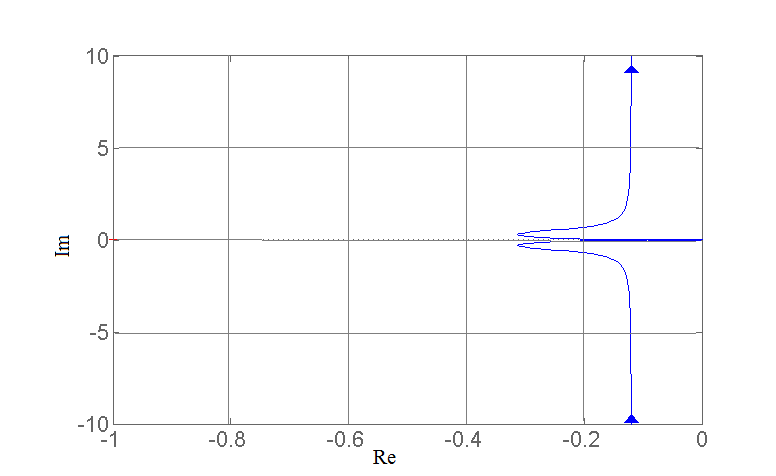
\includegraphics[width = 0.8\textwidth]{2}
	\caption{АФЧХ}
\end{figure}
\newpage
\begin{center}
	\section{Анализ замкнутой системы}
\end{center}


Передаточная функция с коэффициентом обратной связи $K$ записана ниже.
\begin{equation}
W_\text{замк.}(s) = \frac{s + 2}{3s^3 + 4s^2 + (5 + K)s + 5K}
\end{equation} \par
Далее на рисунке 4 представлен графики корней при разных коэффициентах обратой связи $K \in [0, 100]$. \par
\begin{figure} [h!]
	\centering
	\begin{tikzpicture}
	\begin{axis} [
	width = 0.9\textwidth,
	height = 0.5\textwidth,
	xlabel = {Re},
	ylabel = {Im},
	grid = major,
	grid style = {dashed},
	legend pos = north west,
	xmin = -3.1, xmax = 0.8,
	]
	\addplot[mark = none, blue, mark size = 3pt] table [x = Re1, y = Im1] {rlocus.txt};
	\addplot[mark = none, blue] table [x = Re2, y = Im2] {rlocus.txt};
	\addplot[mark = none, blue] table [x = Re3, y = Im3] {rlocus.txt};
	\addplot[only marks, mark = o, mark size = 5pt] coordinates {(-2, 0)};
	\draw[fill] (0, 0) circle (0.07cm);
	\draw[fill] (-0.67, 1.105) circle (0.07cm);
	\draw[fill] (-0.67, -1.105) circle (0.07cm);
	\draw (0, 0) -- (-0.2, 3);
	\draw[] (-0.67, 1.105) -- (-0.2, 3);
	\draw (-0.67, -1.105) -- (-0.2, 3);
	\draw (-0.2, 3) node[anchor = south] {K = 0};
	\legend{полюса, , , нули};
	\end{axis}
	\end{tikzpicture}
	\caption{Нули и полюса}
\end{figure}
Как видно, при $K = 0$ система имеет 1 нулевой корень и находится на границе устойчивости нейтрального типа, при увеличении $K$, система становится устойчивой, при этом вещественная часть комплексно сопряженных корней стемится в правую полуплоскость, что ведет к неустойчивости системы. \par
Пользуясь критерием Гурвица можно вывести, что система будет устойчива при следующих $K$:
\begin{equation}
0 < K < 1.82
\end{equation}
\parЭто также соответствует рисунку 4. Выберем $K = 0.55$ и будем дальше с ним работать.\par
\noindent
\begin{minipage}[t]{0.5\textwidth}
	\begin{figure} [H]
		\centering
		\begin{tikzpicture}
		\begin{axis} [
		width = 0.8\textwidth,
		xlabel = {Re},
		ylabel = {Im},
		grid = major,
		grid style = {dashed},
		legend pos = north west,
		xmin = -3.5, xmax = 0,
		]
		\addplot[only marks, mark = x, mark size = 5pt] coordinates {(-0.34, 1.14) (-0.34, -1.14) (-0.65, 0)}; 
		\addplot[only marks, mark = o, mark size = 5pt] coordinates {(-2, 0)};
		\legend{полюса, нули};
		\end{axis}
		\end{tikzpicture}
		\caption{Нули и полюса}
	\end{figure}
\end{minipage}
\begin{minipage}[t]{0.5\textwidth}
	\vspace{0.5cm}
	\parindent = 15mm
	В таком случае набор корней будет следующим (также корни изображены на рисунке 5):
	\begin{align*}
	p_1 & = -2 & 
	z_1 & =  -0.65 \\
	z_{2, 3} & =  -0.34 \pm 1.14i &
	\end{align*} \par
	Как видно из рисунка 5 система устойчива. Степень устойчивости системы равна $Re(z_2) = Re(z_3) = -0.34$.
\end{minipage}
\newpage
\parНа рисунке 6 и 7 представлены графики переходной и весовой функций замкнутой системы.
\begin{center}
	

\begin{figure}[h]
	\centering
	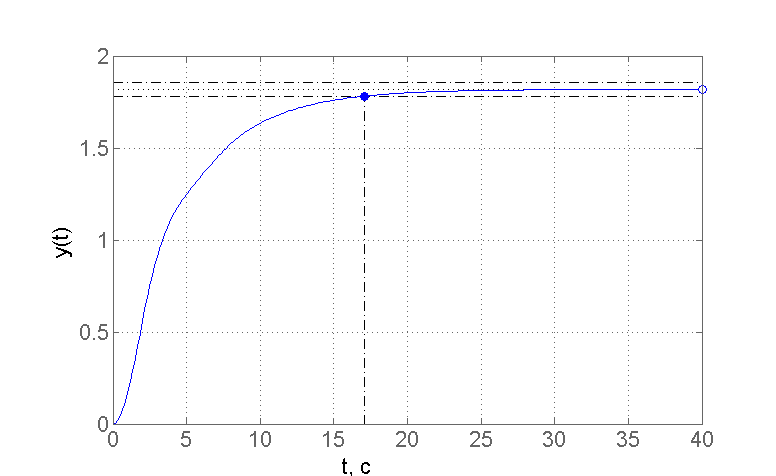
\includegraphics[width = 0.8\textwidth]{1}
	\caption{Переходная функция}
\end{figure}

\begin{figure} [H]
	\begin{tikzpicture}
	\begin{axis} [
	width = \textwidth,
	height = 6cm,
	xlabel = {t, c},
	ylabel = {y},
	grid = major,
	grid style = {dashed},
	xmin = 0, xmax = 25.3,
	xtick = {0, 5, 10, 15, 20, 25},
	ytick = { 0, 0.1, 0.2, 0.3, 0.4}
	]
	\addplot[blue, mark = none] table {impulse.txt};
	\end{axis}
	\end{tikzpicture}
	\caption{Весовая функция} 
\end{figure}
\end{center}
Время переходного процесса $t_\text{п}$ и перерегулирование $\sigma$ угазаны ниже:
\begin{align*}
t_\text{п} & = 17.1 c & \sigma & = 0\%
\end{align*} \par
Далее приведем модель 3 к модели ВСВ. Она выглядит следующим образом:
\begin{equation}
\begin{cases}
\dot{X} = \begin{bmatrix}
0 & 1 & 0 \\
0 & 0 & 1 \\
0 & -\frac{5}{3} & -\frac{4}{3}
\end{bmatrix}X + \begin{bmatrix}
0 \\ 0 \\ 1
\end{bmatrix}U \\
y = \begin{bmatrix}\frac{2}{3} & \frac{1}{3} & 0\end{bmatrix} X
\end{cases}
\end{equation}
где $x = \begin{bmatrix} x_1 & x_2 & x_3 \end{bmatrix}^T$.
\newpage
\par
Теперь можно составить матрицы управляемости $W_y$ и наблюдаемости $W_\text{н}$ для опредления управляемости и наблюдаемости модели.

\begin{align*}
W_y & = \begin{bmatrix}
0 & 0 & 1 \\
0 & 1 & -\frac{4}{3} \\
1 & -\frac{4}{3} & \frac{1}{9} \\
\end{bmatrix} & 
W_\text{н} & = \begin{bmatrix}
\frac{2}{3} & \frac{1}{3} & 0 \\
0 & \frac{2}{3} & \frac{1}{3} \\
0 & \frac{4}{3} & \frac{2}{3} \\
\end{bmatrix}
\end{align*}
\parПоскольку $rang\{W_y\} = 3$ система является управляемой. При этом система является не наблюдаемой, поскольку $rang\{W_\text{н}\} = 2$.

\newpage
\begin{center}
	\section*{Выводы}
\end{center}

В данной работы мы исследовали разомкнутую систему. Получили ее корни и сравнили коренной критерий и Найквиста. Неустойчивая система по Накйквисту является системой на нейтральной границе устойчивости по корневому критерию. Также мы построили ЛАЧХ и ЛФЧХ, и по ним определили запас устойчивости по амплитуде и фазе. \par
Также осуществили анализ замкнутой системы по размокнутой(рисунок 4). При К = 0 система становится разомкнутой. При увеличении К до 0,82 система будет устойчивой. \par

По полученной модели ВСВ мы проверили ее на управляемость и наблюдаемость.Система является управляемой и не наблюдаемой.


\end{document}